%%\documentclass[a4paper, 12pt]{scrreprt}

\documentclass[a4paper, 12pt]{scrartcl}
%usepackage[german]{babel}

%\usepackage{amsmath}
%usepackage{color}
\usepackage[utf8]{inputenc}
\usepackage[T1]{fontenc}
\usepackage{wrapfig}
\usepackage{lipsum}% Dummy-Text

%%%%%%%%%%%%bis hierhin alle nötigen userpackage

\usepackage[utf8]{inputenc}
\usepackage{amsmath}
\usepackage{amsfonts}
\usepackage{amssymb}
\usepackage{graphicx}
%\usepackage{wrapfig}
\usepackage[ngerman]{babel}
\usepackage[left=25mm,top=25mm,right=25mm,bottom=25mm]{geometry}
%\usepackage{floatrow}
\setlength{\parindent}{0em}
\usepackage[font=footnotesize,labelfont=bf]{caption}
\numberwithin{figure}{section}
\numberwithin{table}{section}
\usepackage{subcaption}
\usepackage{float}
\usepackage{url}
\usepackage{fancyhdr}
\usepackage{array}
\usepackage{geometry}
%\usepackage[nottoc,numbib]{tocbibind}
\usepackage[pdfpagelabels=true]{hyperref}
\usepackage[font=footnotesize,labelfont=bf]{caption}
\usepackage[T1]{fontenc}
\usepackage {palatino}
%\usepackage[numbers,super]{natbib}
%\usepackage{textcomp}
\usepackage[version=4]{mhchem}

%\begin{document}

\newcolumntype{L}[1]{>{\raggedright\arraybackslash}p{#1}} % linksbündig mit Breitenangabe
\newcolumntype{C}[1]{>{\centering\arraybackslash}p{#1}} % zentriert mit Breitenangabe
\newcolumntype{R}[1]{>{\raggedleft\arraybackslash}p{#1}} % rechtsbündig mit Breitenangabe

\section{Zusammenfassung}

Die erhaltenen Bindungslängen stimmen gut mit den Literaturwerten überein (siehe Tabelle~\ref{Tab.1}.) 
Die mittels der CCSD-Methode gewonnenen Werte nähern sich besser an den Gleichgewichtsabstand der Literatur an als die mit der B3LYP Methode. Die ermittelten Dissoziationsenergien für das CO Molekül sind wie zu erwarten wesentlich größer gegenüber dem HCl Molekül. Die Werte decken sich jedoch deutlich schlechter mit der Literatur als es bei dem Gleichgewichtsabstand der Fall ist. 


\section{Auswertung}


Die mittels Gaussian erhaltenen Gleichgewichtsabstände wurden in Tabelle~\ref{Tab.1} zusammengetragen. Dabei handelt es sich um den Atomabstand R, welcher bei den jeweiligen minimalsten Energiewerten einer Datenreihe zu finden ist. Die Dissoziationensenergie wurden erhalten, indem der größte Energiewert der Asymptote vom kleinsten Energiewert der Kurve subtrahiert worden ist.

 \begin{table}[H]
 \centering
 
 
 \caption{Berechnete Gleichgewichtsabstände und Dissoziationsenergien von HCl und CO aus den mittels GAUSSIAN erhaltenen Werten  mit der Methode B3LYP und dem Basissatz 6-31G bzw. der Methode CCSD und dem Basissatz 6-31G*.}
 
 
 \begin{tabular}{L{0.1\textwidth}L{0.20\textwidth}C{0.3\textwidth}C{0.20\textwidth}C{0.20\textwidth}}
\multicolumn{2}{c}{}&\multicolumn{1}{c}{Gleichgewichtsabstand R}&\multicolumn{2}{c}{Dissoziationsenergie}\\
 
  Molekül  & Methode &  in Ängstrom &   in Hartree & in kJ/mol \\
  CO  &B3LYP & 1.17 &  0.48&1260 \\
  CO  & CCSD (SCF)&1.11 & 0.49&1290\\
  CO  & CCSD (MP2)&1.15 & 0.59&1550\\
  CO  & CCSD (MP3)&1.13 & 0.55&1440\\
    CO&Literatur&	1.128323&&1077\\

  HCl  &B3LYP& 1.33 &  0.19&498\\
  HCl  & CCSD (SCF)&1.27  & 0.34&892\\
  HCl  & CCSD (MP2)&1.28  & 0.19&498\\
  HCl  & CCSD (MP3)&1.28  & 0.16&420\\
  HCl&Literatur&	1.27455&&429\\

   \multicolumn{4}{c}{https://webbook.nist.gov> und Holemann wiberg 102. Auflage Seite 141}\\
   
   
 \end{tabular}
 \label{Tab.1}
 \end{table}




\begin{table}[htbp]
  \centering
   \caption{Berechnete Gleichgewichtsabstände und Dissoziationsenergien von HCl und CO aus den mittels GAUSSIAN erhaltenen Werten  mit der Methode B3LYP und dem Basissatz 6-31G bzw. der Methode CCSD und dem Basissatz 6-31G*.}
  \begin{tabularx}{\columnwidth}{XL{0.15\textwidth}L{0.20\textwidth}L{0.10\textwidth}L{0.10\textwidth}}
\multicolumn{2}{c}{}&\multicolumn{1}{c}{Gleichgewichtsabstand}&\multicolumn{2}{c}{Dissoziationsenergie}\\
    
      Molekül  & Methode &  R in Ängstrom &   in Hartree & in kJ/mol \\
      \toprule[2pt]
  CO  &B3LYP & 1.17 &  0.48&1260 \\
  CO  & CCSD (SCF)&1.11 & 0.49&1290\\
  CO  & CCSD (MP2)&1.15 & 0.59&1550\\
  CO  & CCSD (MP3)&1.13 & 0.55&1440\\
    CO&Literatur&	1.128323&&1077\\

  HCl  &B3LYP& 1.33 &  0.19&498.0\\
  HCl  & CCSD (SCF)&1.27  & 0.34&892\\
  HCl  & CCSD (MP2)&1.28  & 0.19&498\\
  HCl  & CCSD (MP3)&1.28  & 0.16&420\\
  HCl&Literatur&	1.27455&&429\\
    
  \end{tabularx}
\end{table}



\begin{figure}[ht]
	\centering	
	\begin{minipage}{0.5\textwidth}
	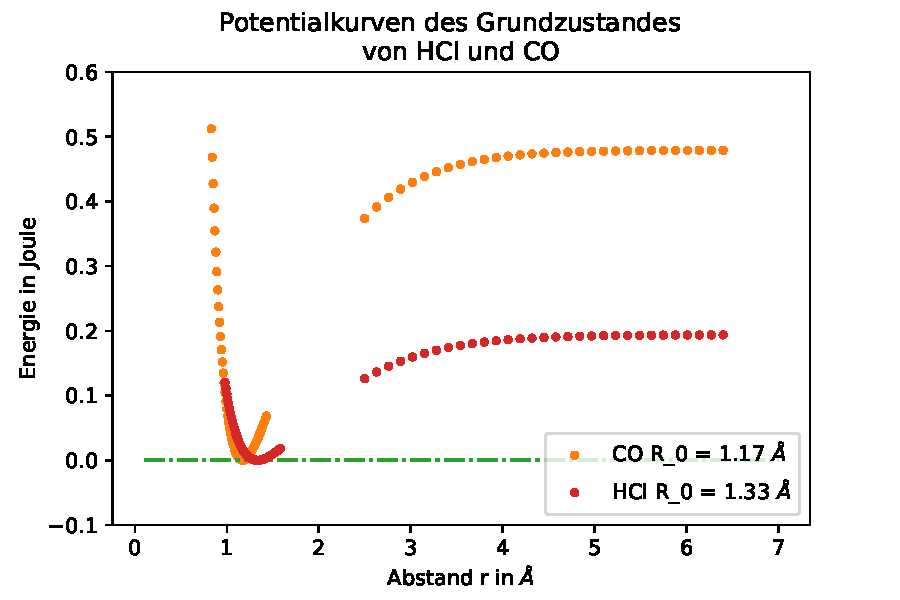
\includegraphics[width=\columnwidth]{Bilder/b3lypzusammen}
	\end{minipage}
	
	
	\caption{Grafische Auftragung der mit der Born-Oppenheimer-Näherung erhaltenen Energien bei verschiedenen Kernabständen von HCl und CO. Die Werte wurden mittels GAUSSIAN mit der Methode B3LYP und dem Basissatz 6-31G erhalten. Die Grafik wurde mit Python erstellt und über Spyder ausgegeben.}
	
	
	\label{b3lypzusammen}
\end{figure}


Wie in Abbildung~\ref{b3lypzusammen} zu sehen beschreiben die mit B3LYP errechneten Werte den Verlauf eines Morsepotentials. Es sei hier erwähnt, dass das tatsächliche Minimum der Kurven nicht bei Null liegt, sondern das Minimum von allen Energiewerten Subtrahiert worden ist, um dieses als Nullpunkt zu definieren. Dadurch ist es nun möglich anhand der Grafen eine qualitative Aussage über die Dissoziationsenergie, sowie den Gleichgewichtsabstand zu machen.


  

 
\begin{figure}[H]
	
\begin{minipage}{0.5\textwidth}
	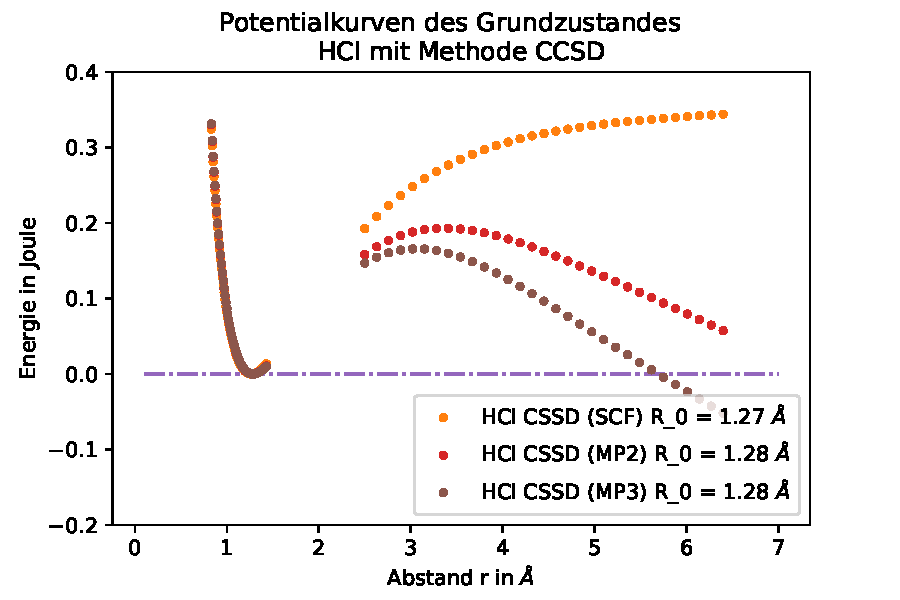
\includegraphics[width=\textwidth]{Bilder/HCl_CCSD}
\end{minipage}
\begin{minipage}{0.5\textwidth}
	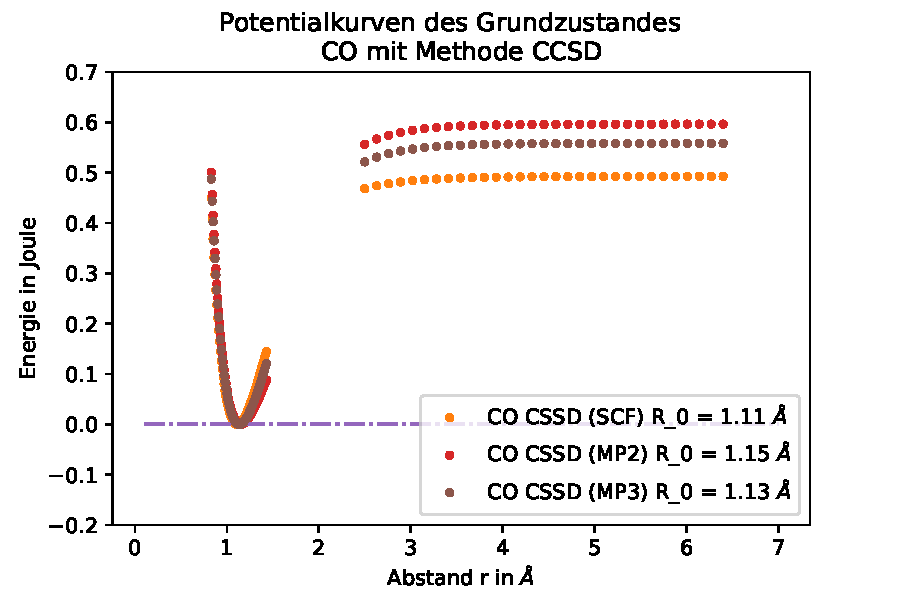
\includegraphics[width=\textwidth]{Bilder/CO_CCSD}
\end{minipage}


\caption{Grafische Auftragung der mit der Born-Oppenheimer-Näherung erhaltenen Energien bei verschiedenen Kernabständen von HCl und CO. Die Werte wurden mittels GAUSSIAN mit der Methode CCSD und dem Basissatz 6-31G* erhalten. Die Grafiken wurde mit Python erstellt und über Spyder ausgegeben.}


	\label{HCl_CCSD}
\end{figure}


Der Verlauf der Werte, welche durch die CCSD Methode für CO, sowie HCl erhalten wurden, sind in Abbildung~\ref{HCl_CCSD} aufgetragen worden. Bei der Betrachtung der Werte kann beobachtet werden, dass die Entwicklung durch Gaussian um das Minimum noch etwas genauer, als es mittels B3LYP der Fall war, gelungen ist. Jedoch beschreibt die Energie  nach der Dissoziation des Moleküle besonders bei HCl einen Verlauf der gänzlich den Erwartungen widerspricht. Die Kurven sollten eigentlich gegen einen Energiewert konvergieren. 






 
 






%\end{document}
